\setlength{\footskip}{8mm}

\chapter{Literature Review} 
\label{ch:literature-review}

\textit{Many efficient techniques based on computer vision are available for classification, object detection, and tracking. Here I review existing work that will be useful for the construction of a wrong-way driving system.}

\section{Background Subtraction }
\label{Background Subtraction}
Background subtraction is a commonly-used technique for generating a foreground mask. In background subtraction, a foreground mask is calculated by subtracting the current frame and a background model obtained with a fixed camera. Every object in the background model is considered as part of the background and is to be ignored.

Background modelling has two main steps:\newline
\tab \hspace{8mm}1. Background initialization.\newline
\tab \hspace{8mm}2. Background update, due to possible changes in the scene.\newline
An example is shown in Figure~\ref{fig:background}.

\begin{figure}[t]
  \centering
  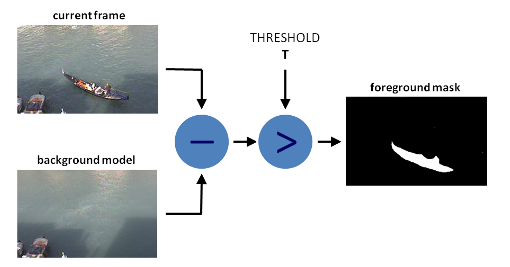
\includegraphics[width=4in]{figures/background.jpg}  
  \caption[Background Subtraction]{Background subtraction example from \shortciteA{itseez2017theopencv}.}
  \label{fig:background}
\end{figure}

Background subtraction is easy to implement, but it is slow, because background subtraction has to perform its calculation over the whole frame on every frame. Large variance in the background can lead to false negatives, and long-term scene change with a slowly-changing background may not work well.



\section{Classification}
\label{Classification}
Classification is a general technique for determining what something is (when we do not know its type) or determining where something is (when the type of object we are looking for is known).

\subsection{Nearest Neighbor Classification}
The nearest neighbor decision rule assigns a label to an unclassified sample point. The classification model simply contains a set of previously-classified points. The nearest neighbor algorithm will find the nearest item in the training set and return the label of that item. This method is simple to implement and powerful, requiring no training time. This classification method usually has the best accuracy, if the training set is large enough, but it requires too much memory and compute time with a large training set. Also, as shown in Figure~\ref{fig:knn}, if a new data item of class 2 is closer to an item of class 1 than any item of class 2, we would classify the input incorrectly. This can be partly addressed by the K-nearest neighbor method. K-nearest neighbor classification allows the user to specify K, the number of stored items to compare against. The method finds the nearest K items in the training set and returns the label of the majority within that group of items. Thus, in Figure~\ref{fig:knn}, if K = 3, The method will classify the new item as a member of class 2.  

\begin{figure}[t]
  \centering
  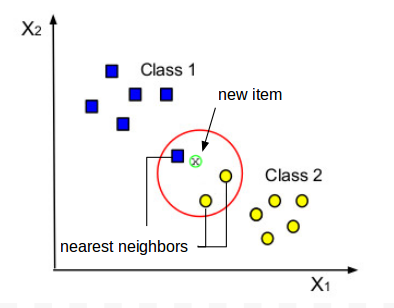
\includegraphics[width=2in]{figures/knn.jpg}   
  \caption[Example of nearest neighbor classification]{Example of nearest neighbor classification.}
  \label{fig:knn}
\end{figure}

\subsection{Support Vector Machines}
A support vector machine (SVM) is a feature-based classifier. Suppose we have a set of given data points, each belonging to one of two classes, and the goal is to decide which class a new data point is in. SVMs use linear hyperplanes for classification. There are many possible hyperplanes that might classify (separate) the training data correctly. Support vector machines choose the unique hyperplane that provides the largest separation of the training data from the hyperplane, as shown for example in Figure~\ref{fig:svm}. When the training data are not linearly separable, the optimization of the hyperplane is more complicated, but still can be modeled as a constrained quadratic optimization. Support vector machines can induce non-linear classification boundaries due to the \textquotedblleft kernel trick" and do not require a large amount of training data.

\begin{figure}[t]
  \centering
  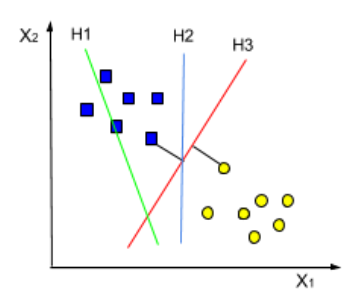
\includegraphics[width=2in]{figures/svm.jpg}   
  \caption[Support Vector Machines]{Example of large margin classification with a linear hyperplane. H1 does not separate the classes. H2 does separate the classes, but with a small margin. H3 separates the classes with a larger margin. }
  \label{fig:svm}
\end{figure}


\subsection{Classical Backpropagation Neural Networks}
Backpropagation is a method for training multi-layer neural networks. Usually, a classical neural network would be feature based. Backpropagation over few layers usually has  similar performance to SVMs. The goal of backpropagation is to optimize a set of weights so that the neural network correctly maps arbitrary inputs to a correct output. The optimization algorithm repeats a two-phase cycle, forward propagation and backward weight update. The input is propagated forward through the network, layer by layer, until it reaches the output layer. The output layer is then compared to the desired output using some loss function. The loss is propagated back from the output layer toward the input layer. This method requires  experimentation to tweak hidden layer size and learning time.

\subsection{Convolutional Neural Networks}
The methods described thus far are normally feature based, requiring the data scientist to mathematically specify the set of features to be extracted from the input data. This is necessary when the training set size is small. For images, CNNs offer the benefit of automatically generated features, offering better performance than feature-based methods so long as a sufficient amount of training data is available.

A CNN usually consists of one or more convolutional layers with subsampling steps followed by one or more fully connected layers. The input to a convolutional layer is a $ m \times n \times r $ image, where $m$ is the height, $n$ is the width, and $r$ is the number of channels in the input. The convolutional layer contains $k$ filters or kernels of size $ p \times p \times q $, where $p$ is smaller than the dimension of the image and $q$ can be the same as the number of channels $(r)$ or smaller and may be different for each kernel. The convolutional units share weights across the entire input image patch. Many open source frameworks such as Caffe allow building of CNNs. An example convolution neural network is shown in Figure~\ref{fig:cnn}.

\begin{figure}[t]
  \centering
  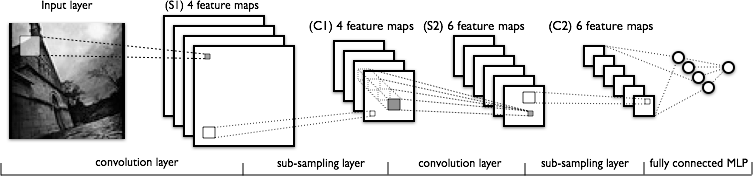
\includegraphics[width=6in]{figures/cnn.jpg}   
  \caption[Example convolutional neural network (CNN)]{Example convolutional neural network (CNN). Reprinted from \shortciteA{deeplearing}.}
  \label{fig:cnn}
\end{figure}



\section{Object Detection}
\label{Object Detection}
Object detection is a very important part of a computer vision system. Detection helps us find objects in an input image. Most detection methods run a scan window over the image and classify each region as a member or not a member of the object class of interest.



\subsection{Haar Cascades}
Object detection using Haar feature-based cascades is one of the most efficient methods to detect an object in the image. Invented by \shortciteA{viola2004robust}, this method requires a medium number of input images (positive images and negative images) for training. After training, we use the resulting model to detect objects in other images.

Positive images are images of an object, and negative images are images without that object. In training, we extract the same set of features from both positive and negative images. Each feature is a single value extracted using a fixed binary kernel as shown in Figure~\ref{fig:haar}.

A large set of possible sizes and locations of each kernel are considered, giving a huge number of possible kernels, making the training process quite heavy. The trained model might contain a large number of features, which would make it correspondingly inefficient. To increase the efficiency of feature computation, integral images are used as a memoization method enabling calculation of sums of intensities across any rectangular region in constant time regardless of block size. 

The new problem is then to find which is a good feature, because a good feature should focus on the essential region and distinctive aspects of the object only. To select features, we use the Adaboost committee-building algorithm. The method applies each and every feature to all training images. For each feature, we find the best threshold for classifying the object as positive or negative over the weighted training set. Each individual feature thus added to the model is a \textquotedblleft weak classifier" that has some level of error over its weighted training set. Different weightings of the training set give different optimal weak classifiers. The best classifier is then a weighted sum of the weak classifiers. 

Applying the resulting complete \textquotedblleft monolithic" committee of weak classifiers to every window in an image will normally achieve good accuracy but is still not a good idea, as it would be unnecessarily computationally intense. To accelerate the computation, we use a cascade of classifiers to group the features into separate stages and apply each stage sequentially. If a window fails in first stage, we do not need to consider it in the remaining stages. Windows that pass though all stages are classified as an instance of the object of interest.

\begin{figure}[t]
  \centering
  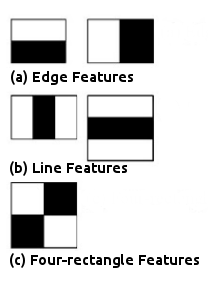
\includegraphics[width=1.5in]{figures/haar.jpg}  
  \caption[Example Haar-like kernels]{Example Haar-like kernels. The sum of the intensities of the pixels in the dark regions is subtracted from those of the light regions. Reprinted from \shortciteA{viola2004robust}. }
  \label{fig:haar}
\end{figure}



\subsection{Histogram of Oriented Gradients}
Histogram of Oriented Gradients (HOG) \cite{dalal2005histograms} is an object detection technique relying on a holistic descriptor of an image patch. HOG generates a representation of the object is contours. Examples of the same object should produce a descriptor as close as possible to the same descriptor calculated when the object is viewed under different conditions. A support vector machine (SVM) is used to recognize HOG descriptors as representing or not representing the object of interest. To recognize objects at different scales, the image is sub-sampled at multiple sizes. Each of these sub-sampled images is then searched to matches. A sample HOG classifier is shown in Figure~\ref{fig:hog}.

\begin{figure}[t]
  \centering
  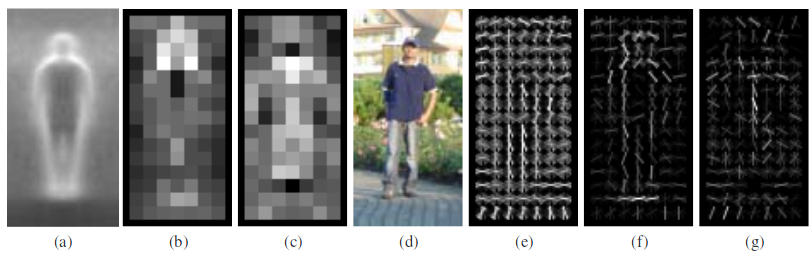
\includegraphics[width=5in]{figures/hog.jpg}  
  \caption[HOG classifier]{HOG classifier. a) The average gradient image over the training examples.  (b) Each “pixel”
shows the maximum positive SVM weight in the block centred on the pixel. (c) Likewise for the negative SVM weights. (d) A test image.
(e) The test image R-HOG descriptor. (f,g) The R-HOG descriptor weighted by respectively the positive and the negative SVM weights. Reprinted from \shortciteA{dalal2005histograms}. }
  \label{fig:hog}
\end{figure}

\subsection{Region-based CNNs}
Region-based CNNs (R-CNNs) \cite{girshick2014rich} combine region proposals with convolutional neural networks (CNNs). When an input image is presented, the system extracts region proposals bottom-up to localize and segment objects. A R-CNN creates region proposals using a process called Selective Search. Selective Search, regardless of the size or aspect ratio of the candidate region, warps the set of pixels in a bounding box around it to a constant size. Once the warped proposals are created, the R-CNN passes them through a convolutional neural network in order to compute features. Once features are extracted and training labels are applied, the R-CNN procedure optimizes one linear SVM per class. Then, for each class, the R-CNN scores each extracted feature vector using the SVM trained for that class. Given all scored regions in an image, R-CNN applies a greedy non-maximum suppression method that rejects regions having an intersection-over union (IoU) overlap with a higher-score selected region larger than a learned threshold. 

R-CNN starts with the ImageNet pre-trained CNN. A SVM training set is created by running the region proposal model over the training set and putting examples with high ground truth IoU into the positive set and other proposals into the negative set. A linear SVM is trained on these positive plus \textquotedblleft hard negative" examples. However, fine tuning such a model on new data turned out to be difficult. When the researchers used the same method of selecting fine tuning examples as they did for the original SVMs, the performance was worse than result with the typical method for fine tuning, in which we update the final softmax layer of the fine-tuned CNN. The softmax classifier was trained on randomly-sampled negative examples rather than on the subset of \textquotedblleft hard negatives" used for SVM training. As result, RCNN uses softmax and random sampling of negatives for fine tuning.

At test time, each region is classified using class-specific linear SVMs. Linear SVMs are used at the output to make it relatively easy to review the classifier model and fine-tune it. The final step is find the tight dimensions of the object bounding box. The R-CNN runs a simple linear regression on the region proposal to generate tighter bounding box coordinates for the final result. This method yields good results, but it requires a large amount of training data and a large amount of compute power. R-CNNs require a forward pass of the CNN for every single region proposal, and we also have to train three different models: the CNN to generate image features, the classifier to predict the class, and the regression model to find the tight dimensions of the candidate object. These factors make R-CNNs slow. An overview of the system is shown in Figure~\ref{fig:rcnn}.

\begin{figure}[t]
  \centering
  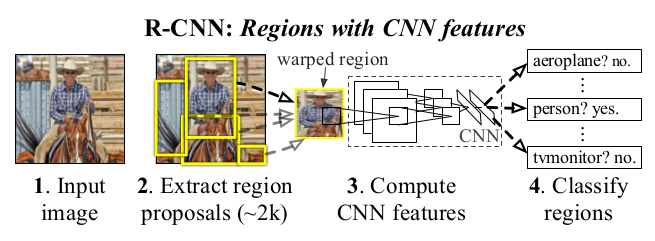
\includegraphics[width=4in]{figures/rcnn.jpg}  
  \caption[Object detection system overview]{Object detection system overview. Reprinted from \shortciteA{girshick2014rich}. }
  \label{fig:rcnn}
\end{figure}

\subsection{FAST R-CNNs}
The Fast Region-based Convolutional Network method (Fast R-CNN) by \shortciteA{girshick2015fast} builds on R-CNNs to improve training and testing speed while also increasing detection accuracy. R-CNNs are slow because they perform a CNN forward pass for each object proposal, without sharing computation. Fast R-CNNs try just run the CNN once per image and share computation over different region proposals. Fast R-CNNs take an input image and multiple regions of interest (RoIs) as input to a fully convolutional network. Each ROI is pooled into a fixed-size feature map and then mapped to a feature vector by fully connected layers. The second thing that Fast R-CNNs do is join the three models of the R-CNN into one model. Fast R-CNNs replace the SVM classifier with a softmax layer on top of the CNN. It also adds a linear regression layer parallel to the softmax layer to output bounding box coordinates. Thus, the network has two output vectors per RoI: a vector softmax probabilities and a vector of per-class bounding-box regression offsets. The architecture of the fast R-CNN is shown in Figure~\ref{fig:fastrcnn}. 

\begin{figure}[t]
  \centering
  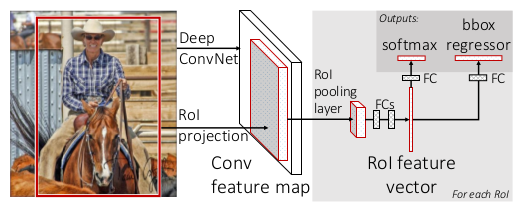
\includegraphics[width=4in]{figures/fastrcnn.jpg}  
  \caption[FAST R-CNNs]{Fast R-CNN architecture. Reprinted from \shortciteA{girshick2015fast}. }
  \label{fig:fastrcnn}
\end{figure}

\subsection{Faster R-CNN}
The faster R-CNN \cite{ren2015faster} is built from previous work especially, the Fast R-CNN and the basic R-CNN. In previous work, the proposals are created using Selective Search, but this is a slow process that was found to be the bottleneck in the overall process. Faster R-CNN introduces a Region Proposal Network (RPN). A RPN is a fully convolutional network that simultaneously predicts object bounds and objectness scores at each position. Faster R-CNN reuses the same CNN results for region proposals instead of running a separate selective search algorithm. See Figure~\ref{fig:fasterrcnn}. The Region Proposal Network works by passing a sliding window over the CNN feature map and at each window, outputting K potential bounding boxes and scores for how good each of those boxes is expected to be. The model then passes each bounding box that is likely to be an object to a Fast R-CNN to generate a classification and tightened bounding boxes as previously described.

\begin{figure}[t]
	\centering
	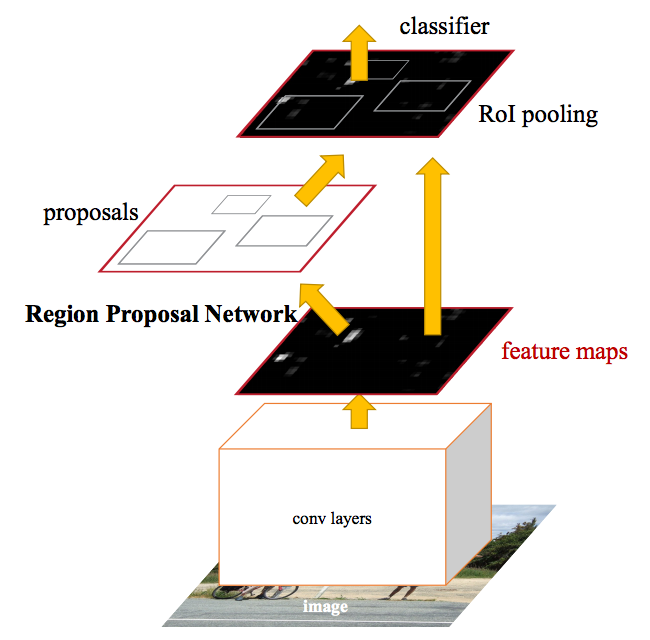
\includegraphics[width=2in]{figures/fasterrcnn.jpg}  
	\caption[Faster R-CNN]{Faster R-CNN. Reprinted from \shortciteA{ren2015faster}. }
	\label{fig:fasterrcnn}
\end{figure}
\begin{figure}[t]
	\centering
	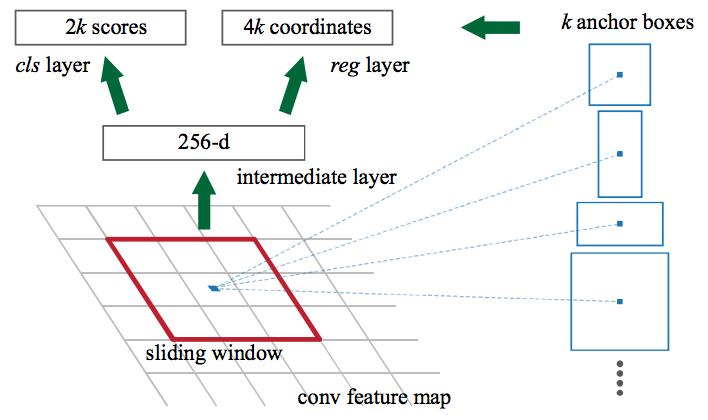
\includegraphics[width=3in]{figures/rpn.jpg}  
	\caption[Region Proposal Network (RPN)]{Region Proposal Network (RPN). Reprinted from \shortciteA{ren2015faster}. }
	\label{fig:rpn}
\end{figure}

\section{Optical Flow} 
\label{Optical Flow}
Optical flow (\shortciteA{horn1981determining}) is a technique used for estimating the motion of moving objects in a scene by keeping track of features between consecutive frames. \textquotedblleft Sparse" optical flow methods start by finding strong corners in the image and then calculating the optical flow for the sparse feature set. The most popular and efficient method is the iterative Lucas-Kanade pyramid method.

Optical flow works on two assumptions:\newline
\tab \hspace{8mm}1. The pixel intensities of an object do not change between consecutive frames.\newline
\tab \hspace{8mm}2. Neighbouring pixels have similar motion.

Consider the motion of a pixel $I(x,y,t)$ (where $t$ is time) that is observed in several consecutive frames. If the object moves by a distance $(dx,dy)$ between two frames taking $dt$ time, under the invariant intensity assumption, we have
\[
\begin{array}{lc}
  {\rm } & {I(x,y,t)} = I(x+dx,y+dy,t+dt). \\ \tag{2.1} \label{eq:2.1}
\end{array}
\]
We perform a Taylor series approximation
\[
\begin{array}{lc}
  {\rm } & {I(x+dx,y+dy,t+dt) \approx I(x,y,t) + \frac{\partial I}{\partial x}dx+\frac{\partial I}{\partial y}d y+\frac{\partial I}{\partial t}dt}.\\ 
\end{array}
\]
From equation \eqref{eq:2.1}, since ${I(x,y,t)} - I(x+dx,y+dy,t+dt) = 0$, dividing by $dt$, we obtain
\[
\begin{array}{lc}
  {\rm } & {\frac{\partial I}{\partial x}\frac{dx}{dt}+\frac{\partial I}{\partial y}\frac{d y}{d t}+\frac{\partial I}{\partial t}\frac{dt}{dt} = 0},\\ 
\end{array}
\]
which we rewrite as
\[
\begin{array}{lc}
  {\rm } & {f_xu + f_yv+ f_t }= 0, \\ 
\end{array}
\]
where
\[
\begin{array}{lc}
  {\rm } & {f_x = \frac{\partial I}{\partial x} \; ; \; f_y = \frac{\partial I}{\partial y} ; \; f_t = \frac{\partial I}{\partial t}}\\ 
\end{array}
\]
\[
\begin{array}{lc}
  {\rm } & {u = \frac{dx}{dt} \; ; \; v = \frac{dy}{dt}.}\\ 
\end{array}
\]
The image gradients are $ f_x $ and $ f_y $. $ f_t $ is a gradient over time. $u$ and $v$ (the motion of the pixel in equation) are unknown. One method to solve this problem is Lucas-Kanade. The Lucas-Kanade method assumes that the spatial displacement of the image content between two successive frames is small. Thus the same optical flow constraints can be assumed to hold for all of the pixels within a window centerd at $p$ (the pixel of interest). Letting $q_1, q_2, \hdots ,q_n$ be the pixels within the window, the common local image flow (velocity) vector $(u,v)$ must approximately satisfy
 \[
 \begin{array}{lc}
 {\rm } & {f_x(q_1)u + f_y(q_1)v} = - f_t(q_1) \\ 
 \end{array}
 \]
\[
\begin{array}{lc}
{\rm } & {f_x(q_2)u + f_y(q_2)v} = - f_t(q_2) \\ 
\end{array}
\]
\[
\begin{array}{lc}
{\rm } & \vdots \\ 
\end{array}
\]
\[
\begin{array}{lc}
{\rm } & {f_x(q_n)u + f_y(q_n)v} = - f_t(q_n). \\ 
\end{array}
\]
These equations can be written in matrix form $A\nu = b$, where
\[
A = \begin{bmatrix}
f_x(q_1) & f_y(q_1)\\
f_x(q_2) & f_y(q_2)\\
\vdots&\vdots\\
f_x(q_n) & f_y(q_n)
\end{bmatrix}
\nu = \begin{bmatrix}
u \\
v
\end{bmatrix}
b= \begin{bmatrix}
-f_t(q_1)\\
-f_t(q_2)\\
\vdots \\
-f_t(q_n)\\
\end{bmatrix}
\]
The least squares solution for $\nu$ can be derived by first transforming the linear system using  
\[
\begin{array}{lc}
{\rm } & {A^TA\nu = A^Tb} \\ 
\end{array}
\]
then obtain,
\[
\begin{array}{lc}
{\rm } &  {\nu = (A^TA)^{-1} A^Tb}, \\ 
\end{array}
\]
where $A^T$ is the transpose of matrix $A$. In a simplified form, we obtain
\[
\begin{array}{lc}
{\rm } & {  \begin{bmatrix} u \\ v \end{bmatrix} = \begin{bmatrix} \sum_{i}{f_{x_i}}^2 & \sum_{i}{f_{x_i} f_{y_i} } \\ \sum_{i}{f_{x_i} f_{y_i}} & \sum_{i}{f_{y_i}}^2 \end{bmatrix}^{-1} \begin{bmatrix} - \sum_{i}{f_{x_i} f_{t_i}} \\ - \sum_{i}{f_{y_i} f_{t_i}} \end{bmatrix}  }.\\ \tag{2.2}
\label{eq:2.2}
\end{array}
\]


According to the assumption that neighbouring pixels must have similar motion, Lucas-Kanade takes a 3 $ \times $ 3 patch around each point. These nine pixels are all assumed to have the same motion, so we calculate  $ (f_x,f_y,$ $ and $ $ f_t) $ for these nine points. We obtain the least squares solution according to the derivation above.

Large motions will be difficult to identify with this method, as the fundamental assumption of small mention is no longer met. Hence, Lucas-Kanade is applied in a pyramid. At higher levels of the pyramid, small motions are ignored, and large motions of large regions become small motions of small regions that can be identified using the same method as above.

\section{Traffic Flow Direction Learning}
\shortciteA{monteiro2007wrongway} present work on a system whose basic idea is to get the correct direction of motion of vehicles in different lanes is during a learning period when it is assumed that traffic is flowing in the correct direction. Hence, the system learns the correct direction for each point in the scene. The authors propose a learning method that analyzes many frames. A Gaussian mixture model is learned for each block in the image by analysis of vehicles' movement over time. This method is good; it is able to detect vehicles circulating on the wrong side of the road, and it runs in real-time. But this method may have errors in identifying objects and may not work well on more crowded scenes. Learning process has shown in Figure~\ref{fig:learning}.
 

\begin{figure}[t]
  \centering
  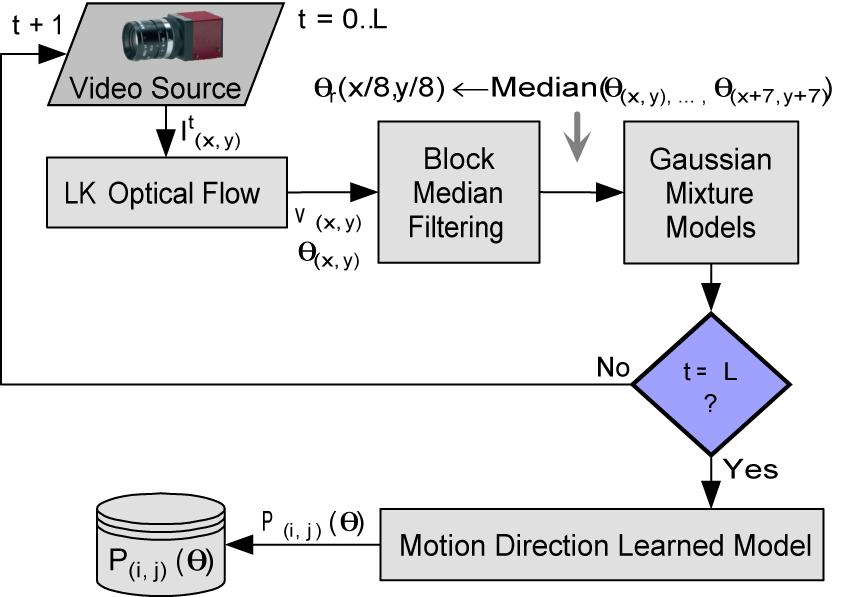
\includegraphics[width=3in]{figures/learning.jpg}  
  \caption[Learning flow chart]{Flow chart of the traffic flow direction learning process. Reprinted from  \shortciteA{monteiro2007wrongway}. }
  \label{fig:learning}
\end{figure}



\section{Object Tracking}
\label{Tracking}
Object tracking has been a problem for research for many years. It is still not a solved problem, but there are many object trackers. Object trackers usually need some initialization step, which can be provided manually or automatically using an object detector. Tracking systems must address two basic problem: motion and matching.
\begin{itemize}
	\item Motion problem: predict the location of an image element using previous positions.
	\item Matching problem: identify the image element within the designated search region.
\end{itemize}

\subsection{CAMSHIFT}
CAMSHIFT is a practical application of the meanshift method to tracking of an object using a color histogram. Meanshift iteratively finds the mode of an arbitrary probability density using samples from the density and a kernel. Consider the situation in which we have a set of points. We are given a small window. The basic idea of meanshift is to identify the set of points that fit with in the small window, then move the window to the area containing the highest density of points. But a problem for the standard meanshift method is that when an object moves closer to camera, the object gets bigger, and vice versa when the camera moves away from the object, making the fixed-size window assumption inapplicable. CAMSHIFT tries to solve this problem by adapting the window size and rotation of the target. It updates the size of the window as $ s = 2 \sqrt{\frac{M_{00}}{256}} $, where $M_{00}$ is the zero-order moment and $ s $ is the new window size. CAMSHIFT also calculates the orientation of the best-fitting ellipse for the object. It applies meanshift with the new scaled search window and a previous window location. The method keeps executing this process until convergence is reached, as measured by a threshold on the shift of the window.

\subsection{Foreground Blob Tracking}
Foreground blob tracking analyzes foreground blobs detected by a background subtraction model. Usually, foreground blob detection is not very accurate, requiring smoothing using a filter such as the Kalman filter.

\subsubsection{Kalman Filter}
A Kalman filter is an optimal estimator for the state of a system evolving stochastically over time. It is an algorithm that uses a series of measurements observed over time and is recursive, so that new measurements can be processed as they arrive. The cycle of a Kalman filter is shown in Figure~\ref{fig:kalman}. Suppose we are tracking a single object. After we detect the object, the detector will give us a candidate location of the object. To predict the next position of the object, we need an object motion model. Furthermore, the detector may not be perfect, so  we assume there is noise in the object location, called measurement noise. The motion model is also not perfect, thus we also assume we will have noise in the motion model, called process noise. To estimate the next position of an object, we need three parameters: the object motion model, the measurement noise, and the process noise.

\textbf{The initial state} of the object must be estimated somehow. Usually, we would use the first detection with the inverse of the sensor model as an initial state. Typically, the state includes the object's position and velocity in 2D or 3D, and the detector gives a noisy estimate of object's  2D or 3D position, usually 2D only. This is the position measurement. Let $x(t)$ be the state vector and, $z(t)$ be the measurement. Given the initial state $x_{0|0}$ and the initial uncertainty about that state expressed as a Gaussian covariance matrix $P_{0|0}$, we begin prediction and correction.

\textbf{Predict} 
is the step of extrapolating the next state using the motion model. Prediction also updates the uncertainty about the object state.
In the state prediction step, an estimate of the next state $ \hat{x}_{t|t-1} $ is obtained by multiplying the previous state estimate by the state transition matrix $(F)$. This prediction can be written as 
\[
\begin{array}{lc}
{\rm } & {\hat{x}_{t|t-1}} = F_t \hat{x}_{t-1|t-1}.  
\end{array}
\]
The covariance prediction is done by multiplying the covariance matrix from the previous iteration by the state transition matrix $F$ and by adding the process noise $Q$, which can be constant $(Q)$ or dynamic $(Q_t)$. The prediction for $P$ is
\[
\begin{array}{lc}
{\rm } & {P_{t|t-1}} = F_t P_{t-1|t-1} F_t^{T}+ Q_{t}.  
\end{array}
\]
\textbf{Correct.} Here we perform a Kalman filter update, which includes a state update and an uncertainty update. First we obtain a noisy measurement $z(t)$. The noise in $z(t)$ is modeled by a single Gaussian covariance matrix $R_t$. To update the state estimate using the measurement, we use the measurement sensor model $H$. We first calculate the prediction error, i.e., the difference between the predicted and observed sensor measurement. This is called the residual or innovation, denoted by $\hat{y}_t$. The innovation or measurement residual is calculated as
\[
\begin{array}{lc}
{\rm } & {\hat{y}_t = z_t - H_t \hat{x}_{t|t-1} ,} 
\end{array}
\]
where $\hat{x}_{t|t-1}$ is the predicted measurement and $z_t$ is the actual measurement. The uncertainty in the innovation residual is 
\[
\begin{array}{lc}
{\rm } & {S_t = H_t P_{t|t-1} H_t^{T} + R_t ,} 
\end{array}
\]
where $P_{t|t-1}$ is the predicted covariance and $R_t$ is the measurement noise the first update uses the Kalman gain matrix $(K)$, which specifies how much we believe the prediction and how much we believe in the measurement. $K_t$ is calculated as 
\[
\begin{array}{lc}
{\rm } & {K_t =  P_{t|t-1} H_t^{T}S_t^{-1} .} 
\end{array}
\]
Clearly, $K_t$ is large if $P_{t|t-1}$ is large and is small if $S_t$ is large. The Kalman gain is now used to update the state $x$ and covariance matrix $P$ according to
\[
\begin{array}{lc}
{\rm } & {\hat{x}_{t|t} =  \hat{x}_{t|t-1} + K_t\hat{y}_{t}} 
\end{array}
\]
\[
\begin{array}{lc}
{\rm } & {P_{t|t} =  (I- K_t + H_t)P_{t|t-1}.} 
\end{array}
\]

When the correction step is finished, we repeat the prediction step, as shown in Figure~\ref{fig:kalmanprocess}. When $K_t$ is large, we \textquotedblleft trust" the innovation more, and if $K_t$ is small, we \textquotedblleft trust" the predicted state more.

\begin{figure}[t]
	\centering
	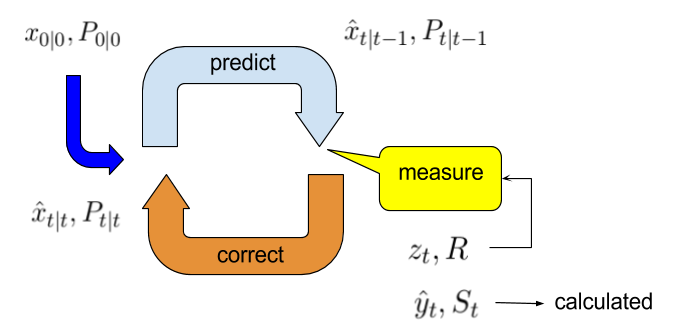
\includegraphics[width=3in]{figures/kalmanprocess.jpg}  
	\caption[Overview of processing by a Kalman filter]{Overview of processing by a Kalman filter. An initial estimated of the state after posterior error distribution care recursively updated as new measurements arrive. }
	\label{fig:kalmanprocess}
\end{figure}

\begin{figure}[t]
	\centering
	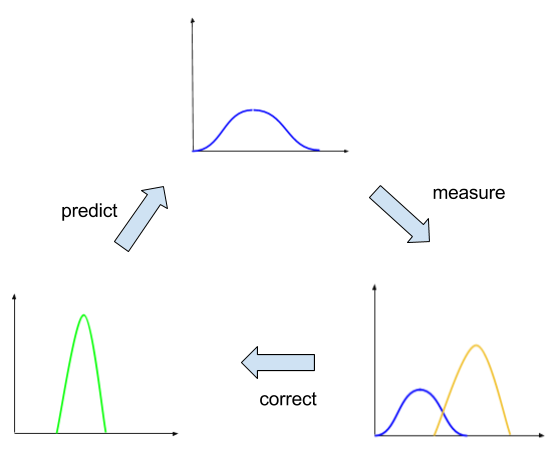
\includegraphics[width=4in]{figures/kalman.jpg}  
	\caption[The cycle of a Kalman filter]{The cycle of a Kalman filter. First the filter predicts the next state from the provided state, then if applicable, the noisy measurement information is incorporated in the correction phase. The cycle is repeated. }
	\label{fig:kalman}
\end{figure}


\FloatBarrier

